\section{Matlab implementation}\label{ch:matlab-implementation}
Both CMOs and the SSMO as defined in Subsections \ref{subsec:CMO-architecture} and \ref{subsec:ssmo-architecture} have been implemented in Matlab. In this chapter the implementations will be discussed and the MOs will be applied on the mass-spring-damper system as described in Chapter \ref{ch:system-definition}. The implementation uses classes for the system, attack, shared multi-observers and the specific multi-observers. All of these will be discussed in this chapter, the code itself can be found in Appendix \ref{ap:matlab-code}.

\subsection{Class explanation}
The system class (\texttt{msd}) defines the system matrices for a mass-spring-damper as in Chapter \ref{ch:system-definition}. The class can creates the state-space system consisting of matrices \eqref{eqn:msd-A}\eqref{eqn:msd-B}\eqref{eqn:msd-E}\eqref{eqn:msd-C}. The class can create both linear and nonlinear systems and works for any number of masses in series.

The \texttt{attack} class defines an attack on the system, the outputs that are to be attacked can be specified. If no outputs are specified, a random selection is made. A list with ones indicating an attack and zeros indicating no attack is made, later on this one is substituted by the attack signal. The specific attack signal can be changed within the \texttt{attackFunction} function.

All MOs are based on a common set of $J$-observers and $P$-observers as defined in Subsection \ref{subsec:state-estimates}. Since all MOs observe the same system, these observers can be defined once and used by all MOs. A separate \texttt{mo} object needs to be generated for both the $J$ and $P$-observers. The \texttt{mo} defines observers for each combination as defined in \eqref{eqn:observer-sets}, based on a given number of outputs for each observer (size of each combination). The class generates an $L$ matrix that places the eigenvalues of $A + LC$ at specified locations. Usually, the size of $C$ does not match the number of outputs $N_O$. The \texttt{mo} class automatically creates a set of outputs based on the provided $C$ where the number of rows matches $N_O$.

\textcolor{red}{2D CMO}

The \texttt{cmo3d} class defines the 3D CMO based on the two \texttt{mo} objects for the $J$ and $P$-observers and the system. It generates the system matrices \eqref{eqn:x3d}\eqref{eqn:A-tilde-3D}\eqref{eqn:F-3d}\eqref{eqn:L-3d}\eqref{eqn:eta-3d} and uses the \texttt{attack} object to create a 3D attack vector that stores the ones and zeros for each specific observer.

The \texttt{ssmo} class defines the SSMO based on the \texttt{mo} objects. It generates the shared system matrices \eqref{eqn:controllable-canonical-form} and all transformation matrices \eqref{eqn:ssmo-transformation}. 

\subsection{Running a simulation}
All MOs can be simulated under the same conditions and the results can be compared. The file \texttt{mainClassScript.m} in Appendix \ref{ap:matlab-code}, generates all MOs and solves the ODEs as in equation \eqref{eqn:standard-system}, \eqref{eqn:cmo-single-J-observer} and \eqref{eqn:cmo-single-P-observer}. Figure \ref{fig:unattacked-system-plot} displays the solution of this ODE for the system as in Example \ref{ex:system}. The observer quickly approaches the system state and the error decays to zero.

\begin{figure}[ht]
    \centering
    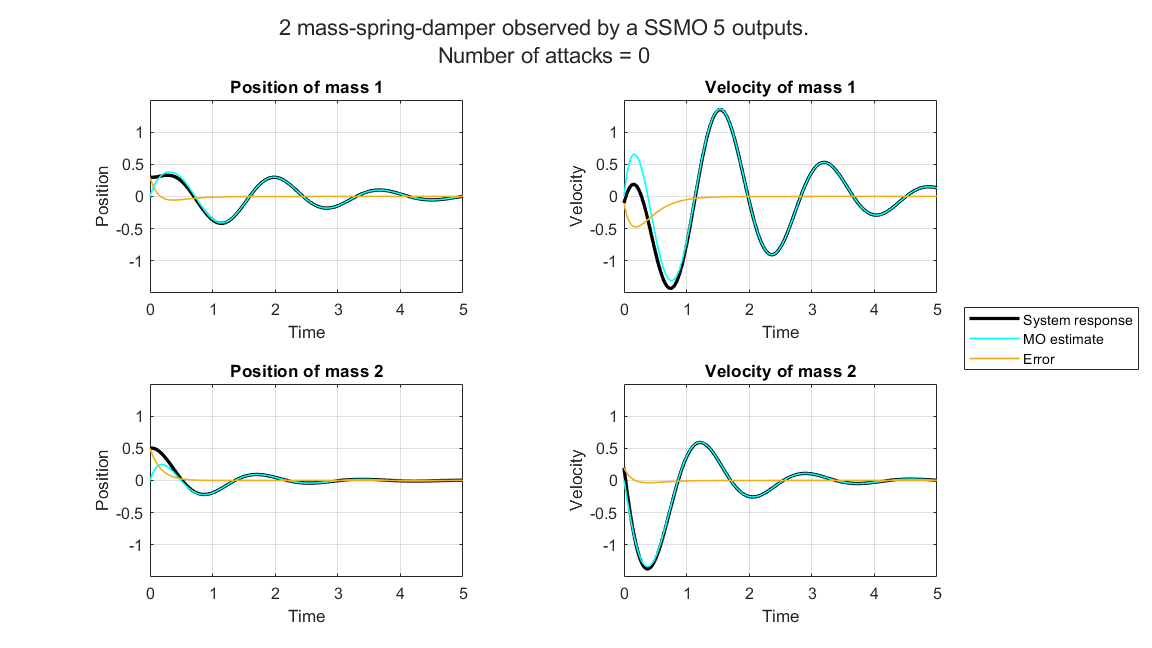
\includegraphics[width=\linewidth]{report/Figures/symplot_5o0a.png}
    \caption{An unattacked, noiseless double mass spring damper and an observer}
    \label{fig:unattacked-system-plot}
\end{figure}

Let us now introduce the attack as in Figure \ref{fig:attack-diagram}, so outputs 2 and 5 are under attack. The attack signal $\tau_j=t,j=2,5$ is injected into both outputs. 

\begin{figure}
    \centering
    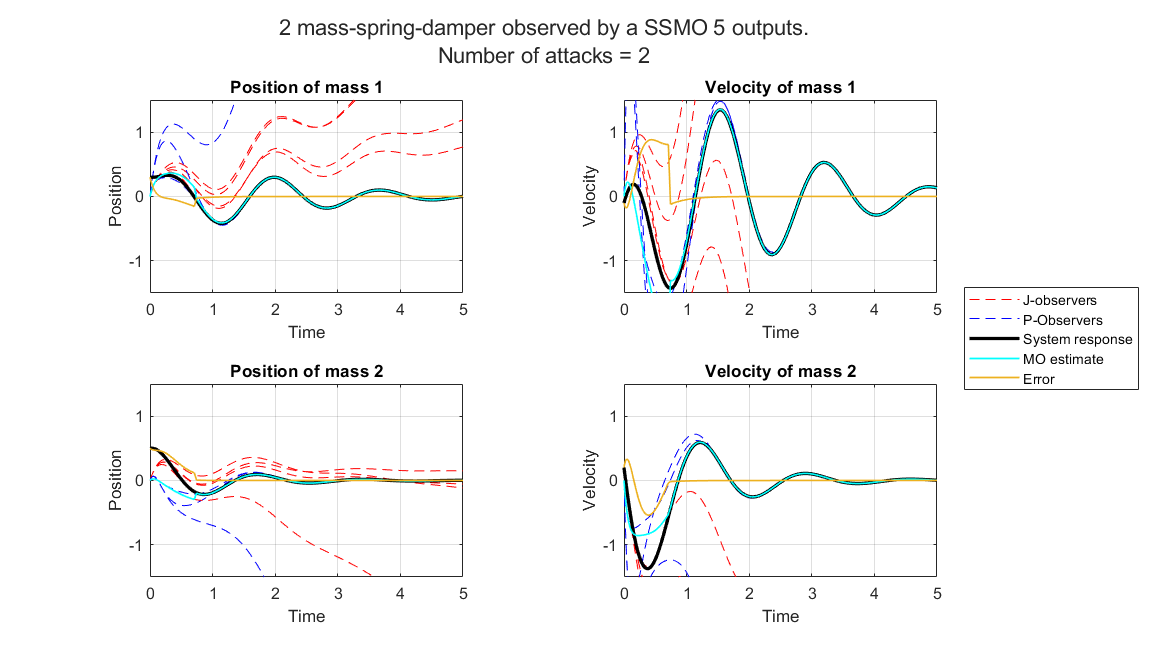
\includegraphics[width=\linewidth]{report/Figures/symplot_5o2a}
    \caption{Caption}
    \label{fig:enter-label}
\end{figure}